\def\layersep{5.5cm}
\def\outsep{0.7cm}
\def\dy{1.25}

\begin{tikzpicture}[draw=black!50, node distance=\layersep, font=\sffamily]
    \tikzstyle{node}=[circle,fill=black,minimum size=2pt,inner sep=0pt]
    \tikzstyle{block}=[draw=black,rectangle,fill=none,minimum size=1.5cm, inner sep=0pt]
    \tikzstyle{annot} = []

	\node[node] (xc) at (0, -\dy cm) {};
	
    \node[block, text width = 2cm, align= center, right=2cm of xc] (CH) {Channel};
    \node[block, text width = 2cm, align= center, right of=CH] (ADC)  {Analog-to-Digital Conveter};
    \node[block, text width = 2cm, align= center, right of=ADC] (EQ)  {Equalizer};
	\coordinate[right=2cm of EQ] (yc) {};
		
    \path[->, >=stealth, shorten >= 0pt] (xc) edge (CH);
    \path[->, >=stealth, shorten >= 0pt] (CH) edge (ADC);
    \path[->, >=stealth, shorten >= 0pt] (ADC) edge (EQ);
    \path[->, >=stealth, shorten >= 0pt] (EQ) edge (yc);
    
    \node[block, draw=none, above = 0.5mm of xc, scale=0.45] (tx_signal) {\resizebox{!}{!}{\begin{tikzpicture}
\begin{axis}[
width=4.52in,
height=3.56in,
scale only axis,
separate axis lines,
every outer x axis line/.append style={white!15!black},
every x tick label/.append style={font=\color{white!15!black}},
xmin=0.00,
xmax=70.00,
ymin=0.00,
ymax=1.00,
xlabel={},
ylabel={},
xmajorgrids,
ymajorgrids,
every outer y axis line/.append style={white!15!black},
every y tick label/.append style={font=\color{white!15!black}},
legend style={draw=white!15!black,fill=white,legend cell align=left}]
\definecolor{matlabColor1}{rgb}{0.000000,0.447000,0.741000}
\addplot [color=matlabColor1, solid, line width=1.5pt, forget plot]
table[row sep=crcr]{
	1 0 \\
	2 0 \\
	3 0 \\
	4 0 \\
	5 0 \\
	6 0 \\
	7 0 \\
	8 0 \\
	9 0 \\
	10 0 \\
	11 0 \\
	12 1 \\
	13 1 \\
	14 1 \\
	15 1 \\
	16 1 \\
	17 1 \\
	18 1 \\
	19 1 \\
	20 1 \\
	21 1 \\
	22 1 \\
	23 0 \\
	24 0 \\
	25 0 \\
	26 0 \\
	27 0 \\
	28 0 \\
	29 0 \\
	30 0 \\
	31 0 \\
	32 0 \\
	33 0 \\
	34 1 \\
	35 1 \\
	36 1 \\
	37 1 \\
	38 1 \\
	39 1 \\
	40 1 \\
	41 1 \\
	42 1 \\
	43 1 \\
	44 1 \\
	45 1 \\
	46 1 \\
	47 1 \\
	48 1 \\
	49 1 \\
	50 1 \\
	51 1 \\
	52 1 \\
	53 1 \\
	54 1 \\
	55 1 \\
	56 0 \\
	57 0 \\
	58 0 \\
	59 0 \\
	60 0 \\
	61 0 \\
	62 0 \\
	63 0 \\
	64 0 \\
	65 0 \\
	66 0 \\
};

\end{axis}
\end{tikzpicture}}};
    \node[block, draw=none, scale=0.45] at ($(CH.east)!0.5!(ADC.west) + (0, 1cm)$) (rx_signal) {\resizebox{!}{!}{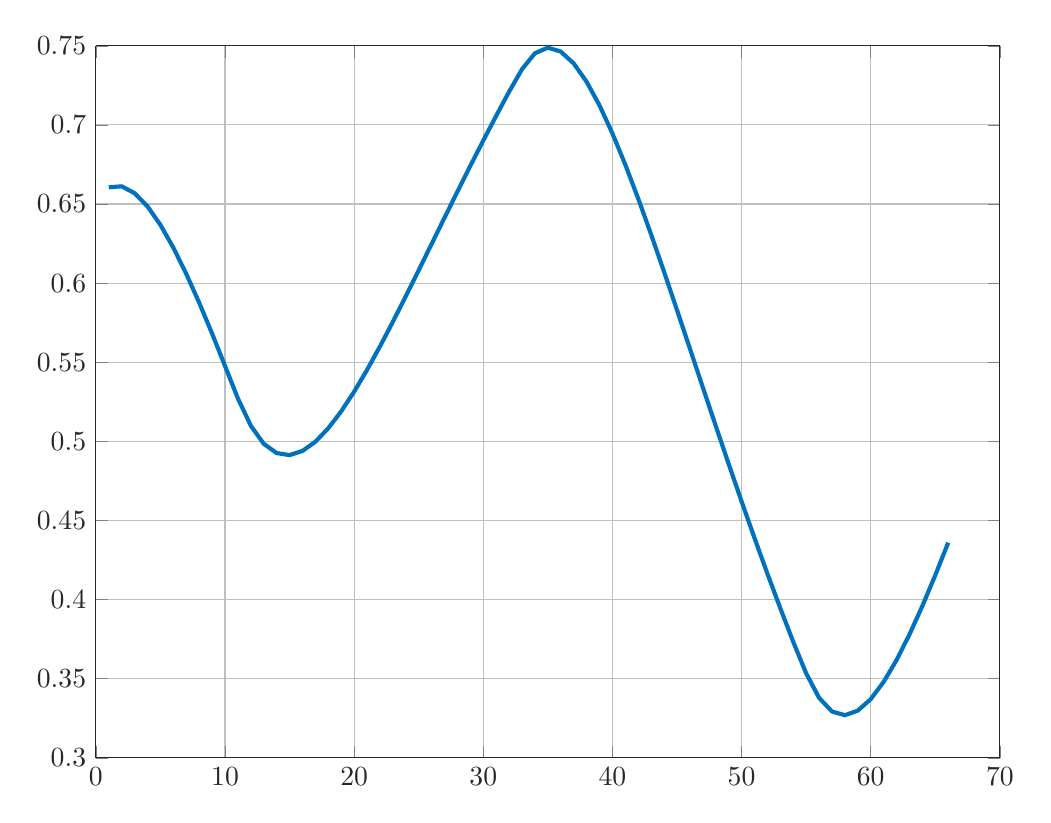
\begin{tikzpicture}
\begin{axis}[
width=4.52in,
height=3.56in,
scale only axis,
separate axis lines,
every outer x axis line/.append style={white!15!black},
every x tick label/.append style={font=\color{white!15!black}},
xmin=0.00,
xmax=70.00,
ymin=0.30,
ymax=0.75,
xlabel={},
ylabel={},
xmajorgrids,
ymajorgrids,
every outer y axis line/.append style={white!15!black},
every y tick label/.append style={font=\color{white!15!black}},
legend style={draw=white!15!black,fill=white,legend cell align=left}]
\definecolor{matlabColor1}{rgb}{0.000000,0.447000,0.741000}
\addplot [color=matlabColor1, solid, line width=1.5pt, forget plot]
table[row sep=crcr]{
	1 0.6606 \\
	2 0.66119 \\
	3 0.65685 \\
	4 0.64848 \\
	5 0.63679 \\
	6 0.6224 \\
	7 0.60585 \\
	8 0.58762 \\
	9 0.56813 \\
	10 0.54763 \\
	11 0.52712 \\
	12 0.50985 \\
	13 0.49845 \\
	14 0.49258 \\
	15 0.49132 \\
	16 0.49395 \\
	17 0.4998 \\
	18 0.50832 \\
	19 0.519 \\
	20 0.53142 \\
	21 0.5452 \\
	22 0.56002 \\
	23 0.57562 \\
	24 0.59174 \\
	25 0.60818 \\
	26 0.62478 \\
	27 0.64139 \\
	28 0.65789 \\
	29 0.67417 \\
	30 0.69016 \\
	31 0.70577 \\
	32 0.72103 \\
	33 0.73522 \\
	34 0.7453 \\
	35 0.74884 \\
	36 0.74634 \\
	37 0.73887 \\
	38 0.72727 \\
	39 0.7123 \\
	40 0.69462 \\
	41 0.67481 \\
	42 0.65334 \\
	43 0.63065 \\
	44 0.60709 \\
	45 0.58298 \\
	46 0.55858 \\
	47 0.53412 \\
	48 0.50978 \\
	49 0.48573 \\
	50 0.46207 \\
	51 0.43893 \\
	52 0.41638 \\
	53 0.39451 \\
	54 0.37328 \\
	55 0.35341 \\
	56 0.33794 \\
	57 0.32928 \\
	58 0.32694 \\
	59 0.32982 \\
	60 0.33708 \\
	61 0.34795 \\
	62 0.36176 \\
	63 0.37793 \\
	64 0.39597 \\
	65 0.41544 \\
	66 0.43596 \\
};

\end{axis}
\end{tikzpicture}}};
	\node[block, draw=none, scale=0.45] at ($(ADC.east)!0.5!(EQ.west) + (0, 1cm)$) (rx_signal_sampled) {\resizebox{!}{!}{\input{figs/rx_waveform_bad_sampled.tex}}};	\node[block, draw=none, above = 0.5mm of yc]  (detected) {010110};

\end{tikzpicture}